% beautiful title slides in Beamer
% Model 6
% latex-beamer.com

\documentclass[aspectratio=169]{beamer}

\usepackage{media9}
\usepackage[backend=bibtex, style=authoryear, doi=false,isbn=false,url=false]{biblatex}
\usepackage[most]{tcolorbox}
\usepackage{subcaption}
\usepackage{bm}
\usepackage{diffcoeff}

% Math macros
\renewcommand\d{\ensuremath{\mathrm{d}}}

\DeclareMathOperator*{\grad}{grad}
\DeclareMathOperator*{\Grad}{Grad}
\DeclareMathOperator*{\Div}{Div}
\renewcommand{\div}{\operatorname{div}}

\newcommand{\bbR}{\mathbb{R}}
\newcommand{\bbF}{\mathbb{F}}
\newcommand{\bbA}{\mathbb{A}}
\newcommand{\bbB}{\mathbb{B}}
\newcommand{\bbS}{\mathbb{S}}

\DeclareMathOperator{\tr}{tr}

\newcommand*{\dual}[1]{\ensuremath{\widehat{#1}}}
\newcommand*{\norm}[1]{\ensuremath{\left\|#1\right\|}}
\newcommand{\where}{\qquad \text{where} \qquad}

\newcommand{\inpr}[3][]{\ensuremath{\langle #2, \, #3 \rangle_{#1}}}
\newcommand{\dualpr}[3][]{\ensuremath{\langle #2 \, \vert #3 \rangle_{#1}}}

\newcommand{\pder}[2]{\ensuremath{\partial_{#2} #1}}
\newcommand{\dder}[2]{\ensuremath{\delta_{#2} #1}}

% Remove navigation bar
%\setbeamertemplate{navigation symbols}{}
\addtobeamertemplate{navigation symbols}{}{%
	\usebeamerfont{footline}%
	\usebeamercolor[fg]{footline}%
	\hspace{1em}%
	\insertframenumber/\inserttotalframenumber
}

\usepackage{color}
\definecolor{theme}{RGB}{0,73,114}

\setbeamertemplate{blocks}[rounded][shadow]

\setbeamercolor{block body alerted}{bg=alerted text.fg!10}
\setbeamercolor{block title alerted}{bg=alerted text.fg!20}
\setbeamercolor{block body}{bg=structure!10}
\setbeamercolor{block title}{bg=structure!20}
\setbeamercolor{block body example}{bg=green!10}
\setbeamercolor{block title example}{bg=green!20}
% Tikz package
\usepackage{tikz}
\usetikzlibrary{positioning}




\graphicspath{{./images/}}

\bibliography{biblio}


%% At begin of each section: show current section and all subsections in the section if any
%% At begin of each subsection except first: show only the current section/subsection
\newif\iftocsub
\tocsubtrue
\AtBeginSection[] {
	\begin{frame}[noframenumbering]{Outline}
		\tableofcontents[sectionstyle=show/shaded, subsectionstyle=show/show/hide]
	\end{frame}
	\tocsubfalse
}
\AtBeginSubsection[] {
	\iftocsub
	\begin{frame}[noframenumbering]{Outline}
		\tableofcontents[currentsubsection, sectionstyle=show/shaded, subsectionstyle=show/shaded/hide]
	\end{frame}
	\fi
	\tocsubtrue
}

\newcommand{\beginbackup}{
	\newcounter{framenumbervorappendix}
	\setcounter{framenumbervorappendix}{\value{framenumber}}
}
\newcommand{\backupend}{
	\addtocounter{framenumbervorappendix}{-\value{framenumber}}
	\addtocounter{framenumber}{\value{framenumbervorappendix}} 
}

\begin{document}
	



% Title slide frame
\begin{frame}[plain]

%%%%%%%% Title slide details %%%%%%%%%%%%%%


% Background Image
\newcommand{\myBackground}
{
    
\includegraphics[height=1.02\paperheight,page=9]{beamerthemeutresources}
}

% Title
\newcommand{\myTitle}
{
    Numerics for the Portwings project
}

% Subtitle
\newcommand{\mySubTitle}
{
    Current develpments and outlook
}

% Author
\newcommand{\myAuthor}   
{
    Andrea Brugnoli
}

% Affiliation
\newcommand{\myAffiliate}
{
  
}

% Presentation Date
\newcommand{\myDate}   
{
    \today
}

% Logo
\newcommand{\myLogo}   
{
    
\includegraphics[width=3cm]{Logo.png}
}
%%%%%%%%%%%%%%%%%%%%%%%%%%%%%%%%%%%%


%%%%%%%%%% Title slide code %%%%%%%%%%%
\begin{tikzpicture}[remember picture,overlay]

% Background color

\fill[white] (current page.south west) rectangle (current page.north east);
% Background image
\node[above right,inner sep=0pt] at (current page.south west)
    {
        \myBackground
    };
    
% Title & Subtitle
\node
[
    above=0.5cm,
    align=center,
    draw=black!50,
    % rounded corners,
    double,
    double distance=0.1cm,
    double=blue!10,
    fill=yellow!10,
    inner xsep=15pt,
    inner ysep=10pt, 
    minimum width=0.7\textwidth,
    text width=0.6\textwidth
] (title) at (current page.center)
{
    \LARGE \myTitle  \\[5pt]
    \small \mySubTitle
};

% Author 
\node[ below=0.5cm] (author) at (title.south){\myAuthor};

% Author 
\node[ below=0.25cm ](affiliate) at (author.south){\small \myAffiliate};

% Date
\node[below=0.25] (date) at (affiliate.south){\large \myDate};

% Logo
\node
[
    below =0.25cm
] at (date.south)
{
    \myLogo
};

\end{tikzpicture}
    
\end{frame}

\begin{frame}{Overview}
	\tableofcontents
\end{frame}

\section{Introduction}

\begin{frame}{Vision for the portwings project}

\begin{block}{Main objective}
Use a unified port-Hamiltonian (pH) framework to model fluid-structure interactions.
\end{block}

If successful, the approach will: 
\begin{itemize}
	\item be competitive w.r.t. state of the art methods;
	\item pave the way to other multiphysical problems;
	\item serve for model reduction and control of complex systems.
\end{itemize}

\begin{figure}[t]
	\begin{subfigure}[t]{0.3\textwidth}
		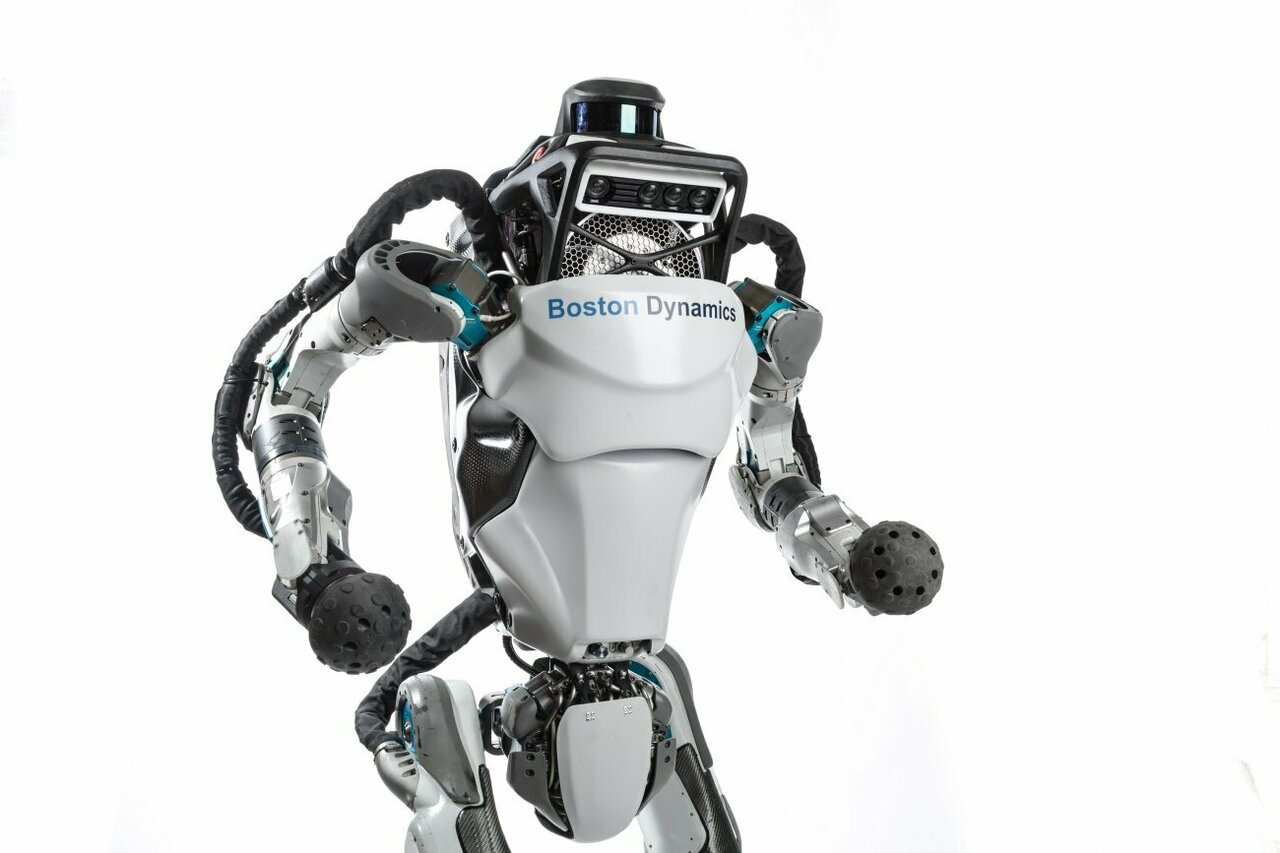
\includegraphics[width=\columnwidth]{robotics.jpg}\\
		\centering{Robotics}%
	\end{subfigure}\hfill
	\begin{subfigure}[t]{0.3\textwidth}
		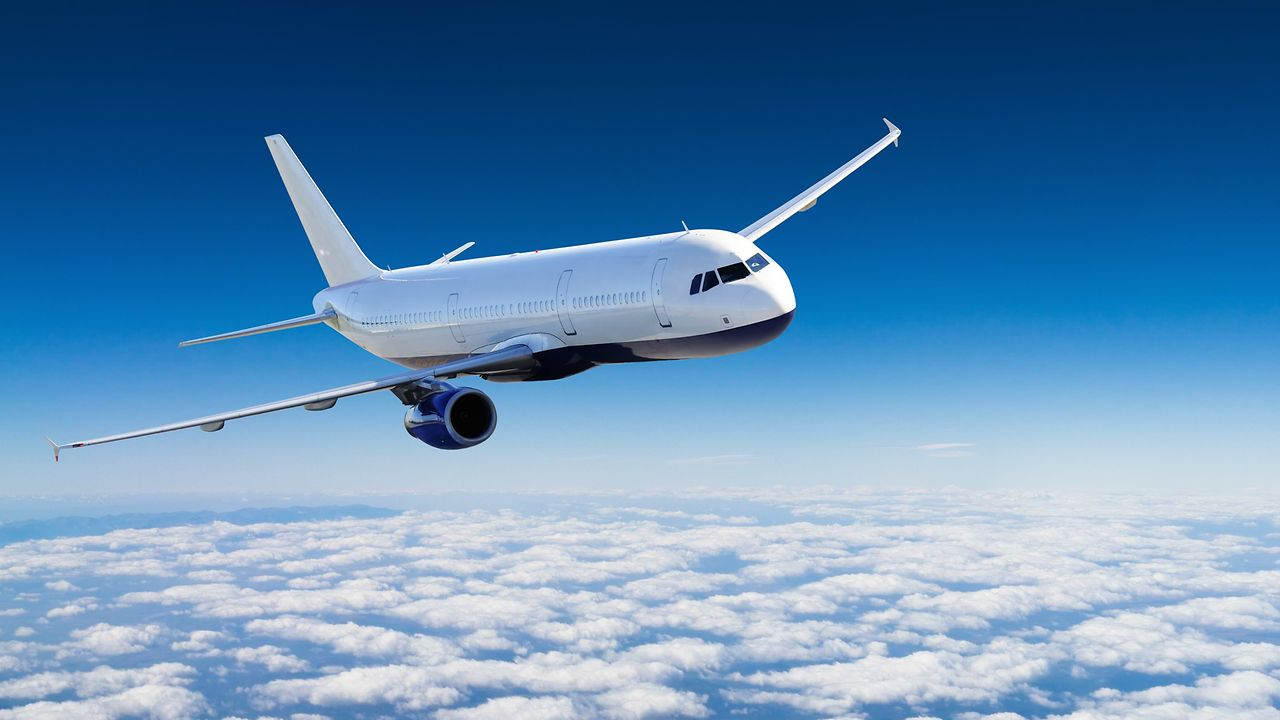
\includegraphics[width=\columnwidth]{aerospace.jpg}\\
		\centering{Aerospace} 
	\end{subfigure}\hfill
	\begin{subfigure}[t]{0.3\textwidth}
		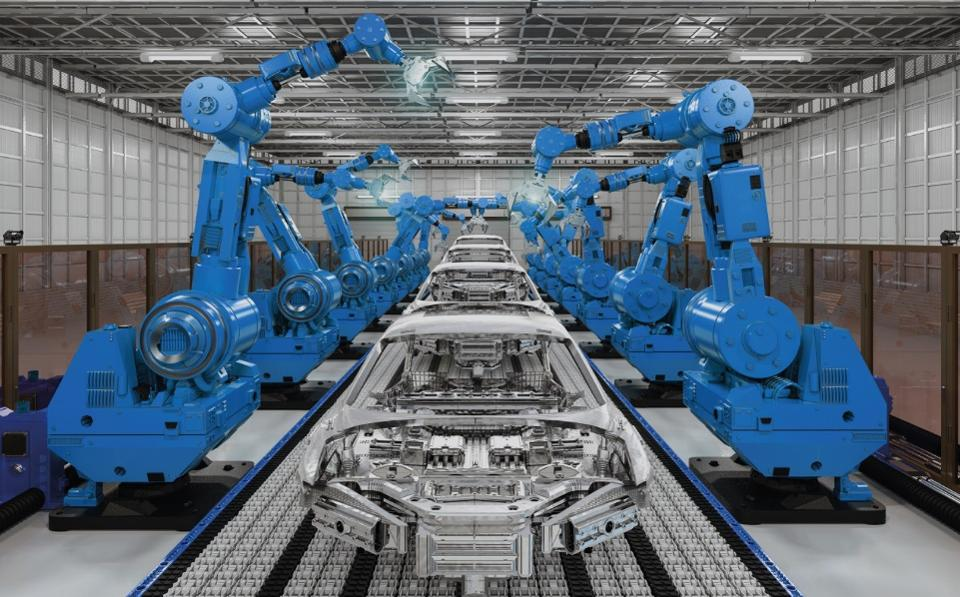
\includegraphics[width=\columnwidth]{manufacturing.jpg}\\
		\centering{Manufacturing}
	\end{subfigure}
\end{figure}

	
\end{frame}

\begin{frame}{The portwings project and its numerical challenges}
	Numerical methods for port-Hamiltonian system should:
	\begin{itemize}
		\item preserve the modularity inherited from the Dirac structure;
		\item reproduce the physical properties of the problem (conservation laws, symmetries);
		\item distinguish between the dynamics and the constitutive equations;
		\item work in any spatial dimension and coordinate frame;
		\item adaptable to many physical problems (fluid and solid mechanics, electromagnetism, etc.);
	\end{itemize}
\end{frame}

\begin{frame}{Methods for computational simulation}
	\only<1>{
\begin{tcbraster}[raster columns=3, raster equal height]
	\begin{tcolorbox}[width=0.32\textwidth, nobeforeafter, colframe=theme,title=Finite differences]%%
	Taylor expansion of derivative
	\begin{itemize}
		\item[\textcolor{green}{\checkmark}] quadrature-free implementation;
		\item[\textcolor{green}{\checkmark}] diagonal mass matrices;
		\item[\textcolor{red}{$\times$}] solution is only pointwise;
		\item[\textcolor{red}{$\times$}] difficult bcs. implementation;
		\item[\textcolor{red}{$\times$}] no Galerkin orthogonality;
	\end{itemize}
	\end{tcolorbox} 
	\begin{tcolorbox}[width=0.32\textwidth, nobeforeafter,  colframe=theme,title=Finite volumes]%%
		Integral form of the equations
		\begin{itemize}
			\item[\textcolor{green}{\checkmark}]  exact discrete conservation laws;
			\item[\textcolor{green}{\checkmark}]  discontinuous phenomena;
			\item[\textcolor{red}{$\times$}] low order approximation;
			\item[\textcolor{red}{$\times$}] requires Delaunay triangulation;
		\end{itemize}
	\end{tcolorbox}
	\begin{tcolorbox}[width=0.32\textwidth, nobeforeafter,  colframe=theme,title=Finite elements]%%
		Variational formulation of the PDE
		\begin{itemize}
			\item[\textcolor{green}{\checkmark}] Galerkin orthogonality;
			\item[\textcolor{green}{\checkmark}] high order elements;
			\item[\textcolor{green}{\checkmark}] mathematical foundation;
			\item[\textcolor{red}{$\times$}] trouble at high aspect ratio;
			\item[\textcolor{red}{$\times$}] convection problems;
		\end{itemize}
	\end{tcolorbox}
\end{tcbraster}
}

\only<2>{
	If the constructions stem from the same ideas, these schemes may be completely equivalent:\\
	\vspace{.5cm}
	\fullcite{adler2021}
	\vspace{1cm}
	
	There is no established superior method and all these methods can all provide impressive results.
}
\end{frame}


\begin{frame}{Finite difference implementation of Rayleigh-Taylor instability}
	\begin{figure}
		\centering
		\includemedia[
		label=vidNoRod,
		addresource=/home/andrea/Videos/Videos_PW/Rayleight_Taylor_FDM.mp4,
		activate=pageopen,
		width=10cm, height=5.5cm, 
		flashvars={
			source=/home/andrea/Videos/Videos_PW/Rayleight_Taylor_FDM.mp4
			&loop=true
		}
		]{}{VPlayer.swf}
	\end{figure}
	Source: \url{https://wci.llnl.gov/simulation/computer-codes/miranda}
\end{frame}


\begin{frame}{Combined finite volume and finite element simulation of a flexible wing}
	\begin{figure}
		\centering
		\includemedia[
		label=vidNoRod,
		addresource=/home/andrea/Videos/Videos_PW/flapping.mp4,
		activate=pageopen,
		width=10cm, height=5.5cm, 
		flashvars={
			source=/home/andrea/Videos/Videos_PW/flapping.mp4
			&loop=true
		}
		]{}{VPlayer.swf}
	\end{figure}
	\fullcite{farhat2012}
\end{frame}

\begin{frame}{Finite elements for computational biology}
	\begin{figure}
		\centering
		\includemedia[
		label=vidNoRod,
		addresource=/home/andrea/Videos/Videos_PW/aorta_FEM.mp4,
		activate=pageopen,
		width=10cm, height=5.5cm, 
		flashvars={
			source=/home/andrea/Videos/Videos_PW/aorta_FEM.mp4
			&loop=true
		}
		]{}{VPlayer.swf}
	\end{figure}
	\fullcite{laadhari2017}
\end{frame}

\begin{frame}{What to choose for port-Hamiltonian systems?}
	Papers concerned port-Hamiltonian systems have tried them all:
	\begin{itemize}
		\item Finite elements (exterior calculus\footcite{golo2004hamiltonian,kotyczka2018weak} or vector calculus\footcite{cardoso2020pfem});
		\item Finite volumes\footcite{serhani2017master};
		\item Finite differences\footcite{trenchant2018};
	\end{itemize}
	\vspace{.5cm}
	\onslide<2->{Two important questions:
	\begin{itemize}
		\item Many of these require an implementation from scratch. Do we really need that?
		\item Can we rely on established theoretical results to have a clear guideline and unified analysis of different methods?
	\end{itemize}}
	
\end{frame}



\section{A unified discretization framework for port-Hamiltonian systems}


\begin{frame}{Exterior calculus and discretization of PDEs}
	
\begin{block}{A unified discretization framework}
	\fullcite{arnold2006acta}
\end{block}

This framework comes with a periodic table of finite elements for unified analysis\footnote{\url{https://sinews.siam.org/Details-Page/periodic-table-of-the-finite-elements}}.

\centering
\includegraphics[width=10cm, height=4cm]{periodic-table-of-the-finite-elements.pdf}
\end{frame}

\begin{frame}{The impact of FEEC}
		\begin{block}{On the importance of FEEC}
			\textit{"Just as the arrangement of the chemical elements in a periodic table led to the discovery of new elements, the periodic table of finite elements has not only clarified existing elements but also highlighted holes in our knowledge and led to new families of finite elements suited for certain purposes."}
		\end{block}
		Two open source libraries were built to implement the FEEC periodic table\footcite{logg2012,rathgeber2017firedrake}.

\end{frame}

\begin{frame}{Some families from the periodic table}
The $\mathcal{P}^-_1\Lambda^k$ family (Whitney forms 1957)
\begin{figure}[t]
	\begin{subfigure}[t]{0.23\textwidth}
		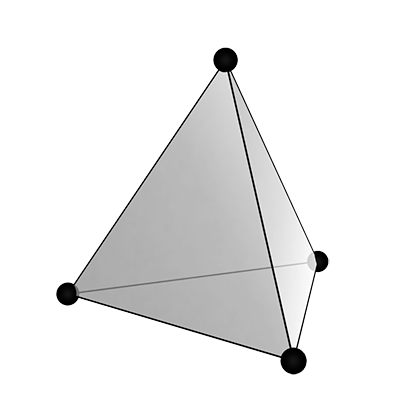
\includegraphics[width=\columnwidth]{P1_tetrahedron.png}%
	\end{subfigure}
	\begin{subfigure}[t]{0.23\textwidth}
		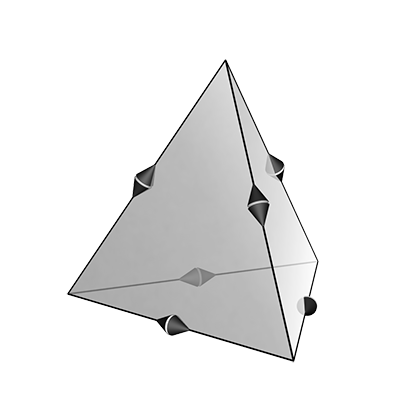
\includegraphics[width=\columnwidth]{N1e1_tetrahedron.png}%
	\end{subfigure}\hfill
	\begin{subfigure}[t]{0.23\textwidth}
		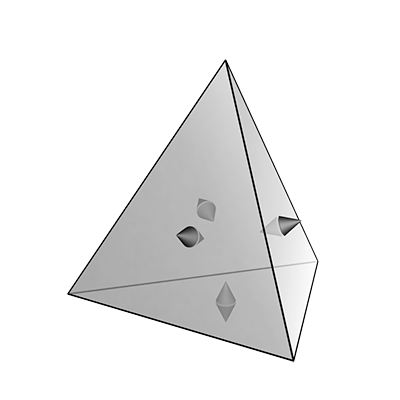
\includegraphics[width=\columnwidth]{N1f1_tetrahedron.png}%
	\end{subfigure}\hfill
	\begin{subfigure}[t]{0.23\textwidth}
		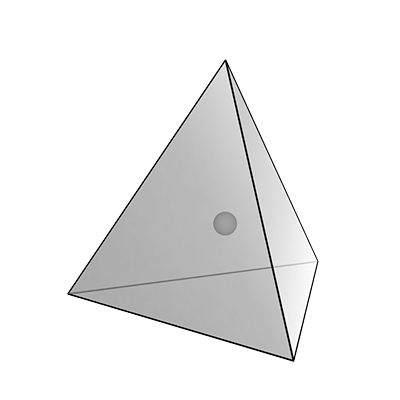
\includegraphics[width=\columnwidth]{dP0_tetrahedron.png}%
	\end{subfigure}\hfill
\end{figure}
The $\mathcal{P}^-_2\Lambda^k$ family
\begin{figure}
	\begin{subfigure}[t]{0.23\textwidth}
		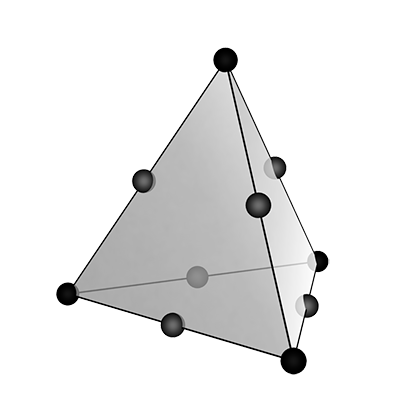
\includegraphics[width=\columnwidth]{P2_tetrahedron.png}%
	\end{subfigure}
	\begin{subfigure}[t]{0.23\textwidth}
		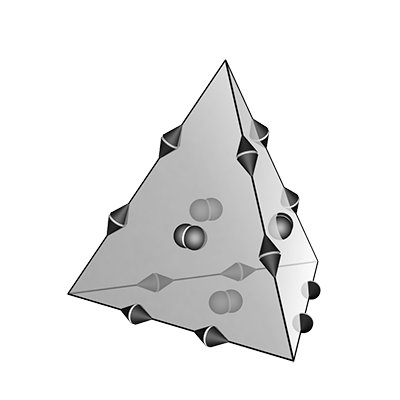
\includegraphics[width=\columnwidth]{N1e2_tetrahedron.png}%
	\end{subfigure}\hfill
	\begin{subfigure}[t]{0.23\textwidth}
		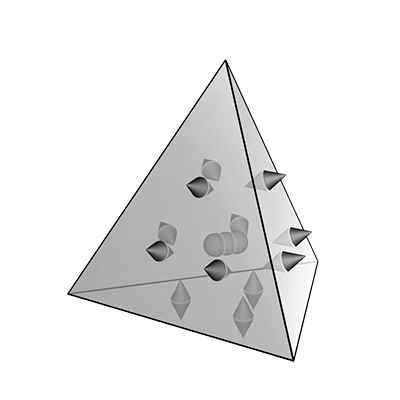
\includegraphics[width=\columnwidth]{N1f2_tetrahedron.png}%
	\end{subfigure}\hfill
	\begin{subfigure}[t]{0.23\textwidth}
		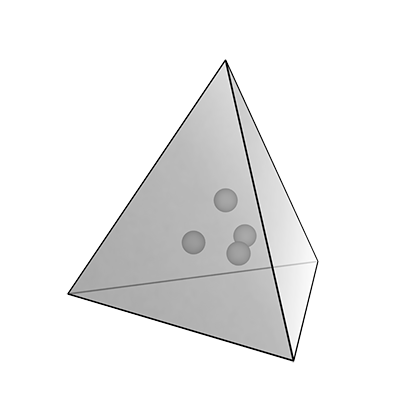
\includegraphics[width=\columnwidth]{dP1_tetrahedron.png}%
	\end{subfigure}\hfill
\end{figure}

\end{frame}


\begin{frame}{On the application of FEEC to port-Hamiltonian systems}

FEEC seems the right way to go to obtain discrete pH models. \\

\begin{alertblock}{Why has this framework not been used (yet)?}
A consistent discretization of pHs raises some difficult points:
\begin{itemize}
	\item \only<2-4>{how to exactly enforce discrete conservation laws?} \only<5->{\textcolor{blue}{how to exactly enforce discrete conservation laws?}}
	\item \only<3-4>{how to obtain discrete constitutive equations (discrete Hodge operator)?}
	\only<5->{\textcolor{blue}{how to obtain discrete constitutive equations (discrete Hodge operator)?}}
	\item<4-> how to implement generic boundary conditions (modular multiphysics modelling)?
\end{itemize}
\end{alertblock}

\end{frame}

\section{Numerical issues in FEM: the illustrative example of the wave equation}


\begin{frame}{The irreducible wave equation}
From the linearization of mass and momentum conservation, the acoustic wave equation in irreducible form is obtained
\begin{equation*}
\frac{1}{\kappa} \diffp[2]{p}{t} - \div\left(\frac{1}{\rho}\grad p\right) = 0,  \qquad \bm{x} \in \Omega \subset \bbR^3, \quad p|_{\partial\Omega} =0,
\end{equation*}
$p$ is the pressure, $\rho$ the density and $\kappa$ the bulk modulus.


\begin{block}{The standard discretization (Dupont 1973)}
	Standard continuous Galerkin scheme:
	\begin{equation*}
		\mathbf{M}_{\kappa^{-1}} \ddot{\mathbf{p}} + \mathbf{K}_{\rho^{-1}} \mathbf{p} = \mathbf{0}.
	\end{equation*}
	What about conservation of energy? Yes, \textcolor{red}{but a Newmark scheme is needed}.\\
	Mass and momentum conservation? \textcolor{red}{Lost (additional analysis required)}.
\end{block}

\end{frame}

\begin{frame}{Maybe the reduction went too far}
\begin{overlayarea}{\textwidth}{\textheight}
	Consider two auxiliary variables
	\begin{equation*}
		v = \partial_t p, \qquad  \bm{\sigma} = \rho^{-1} \grad p, \qquad (v \text{ satisfies } v|_{\partial \Omega}=0),
	\end{equation*}
\only<1>{
two coupled conservation laws (mass and momentum) are obtained
\begin{equation*}
	\begin{bmatrix}
		\kappa^{-1} & 0 \\
		\bm{0} & \rho 
	\end{bmatrix} \diffp{}{t}
\begin{pmatrix}
	v \\ \bm{\sigma}
\end{pmatrix} = 
\begin{bmatrix}
	0 & \div \\
	\grad & \bm{0}
\end{bmatrix}
\begin{pmatrix}
	v \\ \bm{\sigma}
\end{pmatrix}.
\end{equation*}
This system is an Hamiltonian reformulation.
}
\only<2>{
	leading to the discrete weak formulation: find $v_h \in V_h, \; \bm{\sigma}_h \in \Sigma_h$ such that
		\begin{equation*}
		\begin{aligned}
			\inpr[L^2(\Omega)]{\psi_v}{\kappa^{-1}\partial_t v_h} &= \inpr[L^2(\Omega)]{ \psi_v}{\div\bm{\sigma}_h}, \\
			\inpr[L^2(\Omega)]{\bm{\psi}_\sigma}{\rho \partial_t \bm{\sigma}_h} &= \inpr[L^2(\Omega)]{\bm{\psi}_\sigma}{\grad v_h}, \\
		\end{aligned} \qquad
		\begin{aligned}
			\forall \psi_v &\subset V_h, \\
			\forall \bm{\psi}_\sigma &\subset \Sigma_h. \\
		\end{aligned}
	\end{equation*}
\begin{alertblock}{A naive unstable choice}
	Using conforming finite elements (i.e. they can undergo the gradient and the divergence operator resp.)
	\begin{equation*}
		V_h \subset H(\grad, \Omega\vert \; v=0 \text{ on } \partial \Omega):=H^1_0(\Omega), \qquad \Sigma_h \subset H(\div, \Omega).
	\end{equation*} 
the discretization is unstable (stabilized schemes have been devised for this scheme).
\end{alertblock}
}
\end{overlayarea}
\end{frame}

\begin{frame}{The mixed finite element (partial) solution}
\begin{overlayarea}{\textwidth}{\textheight}
One can use integration by parts to obtain a stable discretization.

\only<1>{
	\begin{block}{Mixed $\div$ formulation (Geveci 1988)}
	Find $v_h \in V_h, \; \bm{\sigma}_h \in \Sigma_h$ such that
		\begin{equation*}
			\begin{aligned}
				\inpr[L^2(\Omega)]{\psi_v}{\kappa^{-1}\partial_t v_h} &= +\inpr[L^2(\Omega)]{ \psi_v}{\div\bm{\sigma}_h}, \\
				\inpr[L^2(\Omega)]{\bm{\psi}_\sigma}{\rho \partial_t \bm{\sigma}_h} &= -\inpr[L^2(\Omega)]{\div\bm{\psi}_\sigma}{v_h}, \\
			\end{aligned} \qquad
			\begin{aligned}
				\forall \psi_v &\in  V_h, \\
				\forall \bm{\psi}_\sigma &\in \Sigma_h. \\
			\end{aligned}
		\end{equation*}
		with $V_h\subset L^2(\Omega), \; \Sigma_h \subset H(\div, \Omega)$. \\
		Consequences:
		\begin{itemize}
			\item[\textcolor{green}{\checkmark}] Symplectic schemes guarantee discrete energy conservation;
			\item[\textcolor{green}{\checkmark}] Discrete mass conservation;
			\item[\textcolor{red}{$\times$}] No momentum conservation;
		\end{itemize}
	\end{block}
}

\only<2>{
	\begin{block}{Mixed $\grad$ formulation (Cohen 2000)}
		Find $v_h \in V_h, \; \bm{\sigma}_h \in \Sigma_h$ such that
		\begin{equation*}
			\begin{aligned}
				\inpr[L^2(\Omega)]{\psi_v}{\kappa^{-1}\partial_t v_h} &= -\inpr[L^2(\Omega)]{\grad \psi_v}{\bm{\sigma}_h}, \\
				\inpr[L^2(\Omega)]{\bm{\psi}_\sigma}{\rho \partial_t \bm{\sigma}_h} &= +\inpr[L^2(\Omega)]{ \bm{\psi}_\sigma}{\grad v_h}, \\
			\end{aligned} \qquad
			\begin{aligned}
				\forall \psi_v &\in V_h, \\
				\forall \bm{\psi}_\sigma &\in \Sigma_h, \\
			\end{aligned}
		\end{equation*}
	with $V_h\subset H_0^1(\Omega), \; \Sigma_h \subset L^2(\Omega, \bbR^3)$. \\
		Consequences:
		\begin{itemize}
			\item[\textcolor{green}{\checkmark}] Symplectic schemes guarantee discrete energy conservation;
			\item[\textcolor{green}{\checkmark}] Discrete momentum conservation;
			\item[\textcolor{red}{$\times$}] No mass conservation;
		\end{itemize}
	\end{block}
	
	\Large{Conservation laws cannot be both satisfied!}
}


\end{overlayarea}
\end{frame}

\begin{frame}{Some explanations}
	
	\begin{block}{The Hodge operator and the unstable scheme}
		The instability in the very first formulation is related to a uncorrect discretization of the Hodge operator. \\
		\vspace{.3cm}
		Variables to the left and to right are dual to each other and cannot be discretized using the same spaces!
	\end{block}

	\begin{block}{Failure of discrete conservation laws}
		The integration by parts implies that the conservation law is only weakly satisfied.
	\end{block}

\end{frame}

\section{Dual field discretization of port-Hamiltonian systems}

\begin{frame}{A glimpse of light}
	\fullcite{zhang2021mass}\\
	\vspace{.5cm}
	This article heavily relies on FEEC to obtain the conservation properties.
	\begin{block}{Conservative properties of the dual field approach}
		A dual field discretization essentially used both the $\div$ and $\grad$ mixed formulations
		\begin{itemize}
			\item[\textcolor{green}{\checkmark}] Mass conservation;
			\item[\textcolor{green}{\checkmark}] Momentum conservation;
			\item[\textcolor{green}{\checkmark}] Energy conservation.
		\end{itemize}
		For the Navier Stokes equation the two systems are coupled via the vorticity (convective terms) but a staggered time stepping scheme lead to two \textbf{uncoupled} and \textbf{linear} saddle point problems.
	\end{block}
	
\end{frame}

\begin{frame}{Dual fields discretization and pH systems}
	The dual field discretization naturally applies to pH systems:
	\begin{itemize}
		\item<2-> Mimetically discretize the Dirac structure (fluxes and efforts stay dual);
		\item<3-> Derive an adjoint Dirac structure ($\mathrm{d} \rightarrow \delta$), whose discretization relies on the integration by parts;
		\item<4-> Use both the Hamiltonian from the Dirac structure and its adjoint to get rid of the Hodge operator (no discrete Hodge required for constitutive relations);
		\item<5-> Combine the two systems to reduce the number of unknowns.
	\end{itemize}
\onslide<6->{
\begin{exampleblock}{Benefits of using the dual field for pHs.}
	This approach:
		\begin{itemize}
		\item[\textcolor{green}{\checkmark}] is stable by construction;
		\item[\textcolor{green}{\checkmark}] conserve mass, momentum, energy;
		\item[\textcolor{green}{\checkmark}] does not require topologically dual meshes;
		\item[\textcolor{green}{\checkmark}] can enforce generic boundary conditions in a weak manner (?). 
	\end{itemize}
\end{exampleblock}
}
\end{frame}

\begin{frame}
	
	\Large Any question?
	
\end{frame}

\beginbackup

\begin{frame}{The Whitney forms case: Discrete Stokes Dirac structure}
	Discrete formulation of the Stokes-Dirac structure:\\
$f^p_h \in \mathcal{W}_h^p, \; f^q_h \in \mathcal{W}_h^q$ and $e^p_h \in \mathcal{W}_h^{q-1}, \; e^q_h \in \mathcal{W}_h^{p-1}$
	\begin{equation*}
		\begin{aligned}
			\inpr[M]{v^p}{f^p_h} &= \inpr[M]{v^p}{(-1)^r\d e^q_h}, \\
			\inpr[M]{v^q}{f^q_h} &= \inpr[M]{v^q}{\d e^p_h}, 
		\end{aligned} \qquad
		\begin{aligned}
			f^\partial_h &= \tr e^p_h, \\
			e^\partial_h &=(-1)^p\tr e^q_h. \\
		\end{aligned} \qquad 
		\begin{aligned}
			\forall v^p \in \mathcal{W}_h^p, \\
			\forall v^q \in \mathcal{W}_h^q. \\
		\end{aligned}
	\end{equation*}
Algebraic realisation
\begin{equation*}
	\begin{aligned}
		\begin{bmatrix}
			\mathbf{M}^p & \mathbf{0} \\
			\mathbf{0} & \mathbf{M}^q
		\end{bmatrix}
		\begin{pmatrix}
			\mathbf{f}^p \\
			\mathbf{f}^q
		\end{pmatrix} &=
		\begin{bmatrix}
			\mathbf{0} & (-1)^r\mathbf{M}^p\mathbf{d}^{p-1} \\
			\mathbf{M}^q\mathbf{d}^{q-1} & \mathbf{0}
		\end{bmatrix}
		\begin{pmatrix}
			\mathbf{e}^p \\
			\mathbf{e}^q
		\end{pmatrix}, \\
		\begin{pmatrix}
			\mathbf{f}^\partial \\
			\mathbf{e}^\partial \\
		\end{pmatrix} &= 
		\begin{bmatrix}
			\mathbf{T}^{q-1} & \mathbf{0} \\
			\mathbf{0} & (-1)^p\mathbf{T}^{p-1} \\
		\end{bmatrix}
		\begin{pmatrix}
			\mathbf{e}^p \\
			\mathbf{e}^q
		\end{pmatrix}.
	\end{aligned}
\end{equation*}
\end{frame}


\begin{frame}{The Whitney forms case: Discrete Adjoint Stokes Dirac structure}
	Discrete formulation of the adjoint Stokes-Dirac structure:\\
	$\dual{f}_h^p \in \mathcal{W}_h^{q-1}, \; \dual{f}_h^q \in \mathcal{W}_h^{p-1}, \text{ and } \dual{e}_h^p \in \mathcal{W}_h^{p},  \; \dual{e}_h^q \in \mathcal{W}_h^{q}$ such that
	\begin{equation*}
		\begin{aligned}
			\inpr[M]{\dual{v}^p}{\dual{f}^p_h} &= \inpr[M]{\d\dual{v}^p}{(-1)^{a_0} \dual{e}^q_h} - \dualpr[\partial M]{\dual{v}^p}{(-1)^{b_0} e^q}, \\
			\inpr[M]{\dual{v}^q}{\dual{f}^q_h} &= \inpr[M]{\d\dual{v}^q}{(-1)^{a_1} \dual{e}^p_h} - \dualpr[\partial M]{\dual{v}^q}{(-1)^{b_1} e^p},
		\end{aligned} \qquad 
		\begin{aligned}
			\forall \dual{v}^p \in \mathcal{W}_h^{q-1}, \\
			\forall \dual{v}^q \in \mathcal{W}_h^{p-1}, \\
		\end{aligned}
	\end{equation*}
where $\mathcal{W}_h^k$ is the Whitney forms polynomial space of degree $k$. \\
Algebraic realisation
\begin{equation*}\footnotesize
	\begin{bmatrix}
		\mathbf{M}^{q-1} & \mathbf{0} \\
		\mathbf{0} & \mathbf{M}^{p-1}
	\end{bmatrix}
	\begin{pmatrix}
		\widehat{\mathbf{f}}^p \\
		\widehat{\mathbf{f}}^q
	\end{pmatrix} =
	\begin{bmatrix}
		\mathbf{0} & (-1)^{a_0}\mathbf{d}_{q-1}\mathbf{M}^q\\
		(-1)^{a_1}\mathbf{d}_{p-1}\mathbf{M}^p & \mathbf{0}
	\end{bmatrix}
	\begin{pmatrix}
		\dual{\mathbf{e}}^p \\
		\dual{\mathbf{e}}^q
	\end{pmatrix} -
	\begin{bmatrix}
		\mathbf{0} & (-1)^{b_0}\mathbf{L}_\partial^{p-1} \\
		(-1)^{b_1}\mathbf{L}^{q-1}_\partial & \mathbf{0}
	\end{bmatrix}
	\begin{pmatrix}
		{\mathbf{e}}^p \\
		{\mathbf{e}}^q
	\end{pmatrix}.
\end{equation*}
\end{frame}

\begin{frame}{The General Case (trimmed polynomial space) }

Stokes-Dirac
\begin{equation*}\footnotesize
	\begin{bmatrix}
		\mathbf{M}^p_r & \mathbf{0} \\
		\mathbf{0} & \mathbf{M}^q_r
	\end{bmatrix}
	\begin{pmatrix}
		\mathbf{f}^p \\
		\mathbf{f}^q
	\end{pmatrix} =
	\begin{bmatrix}
		\mathbf{0} & (-1)^r\mathbf{D}^{p-1}_r \\
		\mathbf{D}^{q-1}_r & \mathbf{0}
	\end{bmatrix}
	\begin{pmatrix}
		\mathbf{e}^p \\
		\mathbf{e}^q
	\end{pmatrix}, \qquad
	\begin{pmatrix}
		\mathbf{f}^\partial \\
		\mathbf{e}^\partial \\
	\end{pmatrix} = 
	\begin{bmatrix}
		\mathbf{T}^p_r & \mathbf{0} \\
		\mathbf{0} & (-1)^p\mathbf{T}^q_r \\
	\end{bmatrix}
	\begin{pmatrix}
		\mathbf{e}^p \\
		\mathbf{e}^q
	\end{pmatrix}.
\end{equation*}
Adjoint Stokes-Dirac
\begin{equation*}\footnotesize
	\begin{bmatrix}
		\mathbf{M}^{q-1}_r & \mathbf{0} \\
		\mathbf{0} & \mathbf{M}^{p-1}_r
	\end{bmatrix}
	\begin{pmatrix}
		\widehat{\mathbf{f}}^p \\
		\widehat{\mathbf{f}}^q
	\end{pmatrix} =
	\begin{bmatrix}
		\mathbf{0} & (-1)^{a_0}(\mathbf{D}_r^{q-1})^\top\\
		(-1)^{a_1}(\mathbf{D}_r^{p-1})^\top & \mathbf{0}
	\end{bmatrix}
	\begin{pmatrix}
		\dual{\mathbf{e}}^p \\
		\dual{\mathbf{e}}^q
	\end{pmatrix} -
	\begin{bmatrix}
		\mathbf{0} & (-1)^{b_0}\mathbf{L}_{r, \partial}^{p-1} \\
		(-1)^{b_1}\mathbf{L}^{q-1}_{r, \partial} & \mathbf{0}
	\end{bmatrix}
	\begin{pmatrix}
		{\mathbf{e}}^p \\
		{\mathbf{e}}^q
	\end{pmatrix}.
\end{equation*}

\end{frame}

\begin{frame}{Discrete port-Hamiltonian system}
	Primal pH system
	\begin{equation*}\footnotesize
		\begin{bmatrix}
			\mathbf{M}^p_r & \mathbf{0} \\
			\mathbf{0} & \mathbf{M}^q_r
		\end{bmatrix}
		\begin{pmatrix}
			\dot{{\alpha}}^p \\
			\dot{{\alpha}}^q
		\end{pmatrix} = -
		\begin{bmatrix}
			\mathbf{0} & (-1)^r\mathbf{D}^{p-1}_r \\
			\mathbf{D}^{q-1}_r & \mathbf{0}
		\end{bmatrix}
		\begin{pmatrix}
			\mathbf{e}^p \\
			\mathbf{e}^q
		\end{pmatrix}, \qquad
		\begin{pmatrix}
			\mathbf{u}^p \\
			\mathbf{u}^q \\
		\end{pmatrix} = 
		\begin{bmatrix}
			\mathbf{T}^{q-1}_{r, \Gamma_p} & \mathbf{0} \\
			\mathbf{0} & (-1)^p\mathbf{T}^{p-1}_{r, \Gamma_q} \\
		\end{bmatrix}
		\begin{pmatrix}
			\mathbf{e}^p \\
			\mathbf{e}^q
		\end{pmatrix}.
	\end{equation*}
Adjoint pH system
\begin{equation*}\footnotesize
	\begin{bmatrix}
		\mathbf{M}^{q-1}_r & \mathbf{0} \\
		\mathbf{0} & \mathbf{M}^{p-1}_r
	\end{bmatrix}
	\begin{pmatrix}
		\dot{\dual{\bm{\alpha}}}^p \\
		\dot{\dual{\bm{\alpha}}}^q
	\end{pmatrix} = -
	\begin{bmatrix}
		\mathbf{0} & (-1)^{a_0}(\mathbf{D}_r^{q-1})^\top\\
		(-1)^{a_1}(\mathbf{D}_r^{p-1})^\top & \mathbf{0}
	\end{bmatrix}
	\begin{pmatrix}
		\dual{\mathbf{e}}^p \\
		\dual{\mathbf{e}}^q
	\end{pmatrix} +
	\begin{bmatrix}
		\mathbf{0} & (-1)^{c_0}\mathbf{B}_{r, \Gamma_q}^{p-1} \\
		(-1)^{c_1}\mathbf{B}^{q-1}_{r, \Gamma_p} & \mathbf{0}
	\end{bmatrix}
	\begin{pmatrix}
		{\mathbf{u}}^p \\
		{\mathbf{u}}^q
	\end{pmatrix}. 
\end{equation*}
\end{frame}

\begin{frame}{Incorporation of the constitutive equations (Quadratic case)}

Weak form
\begin{equation*}
	\begin{aligned}
		\inpr[M]{{v}^p}{\alpha^p_h} &= \inpr[M]{{v}^p}{C^p \dual{e}^p_h}, \\
		\inpr[M]{{v}^q}{\alpha^q_h} &= \inpr[M]{{v}^q}{C^q \dual{e}^q_h}, \\ 
	\end{aligned} \qquad 
	\begin{aligned}
		\inpr[M]{\dual{v}^p}{\dual{\alpha}^p_h} &= \inpr[M]{\dual{v}^p}{(-1)^{p(n-p)}\dual{C}^p e^p_h}, \\
		\inpr[M]{\dual{v}^q}{\dual{\alpha}^q_h} &= \inpr[M]{\dual{v}^q}{(-1)^{q(n-q)} \dual{C}^q e^q_h},
	\end{aligned}
\end{equation*}
Algebraic realisation
\begin{equation*}
	\begin{aligned}
		\mathbf{M}_r^p {\alpha}^p &= \mathbf{M}_{C, r}^p \dual{\mathbf{e}}^p, \\
		\mathbf{M}_r^q {\alpha}^q &= \mathbf{M}_{C, r}^q \dual{\mathbf{e}}^q, \\
	\end{aligned} \qquad 
	\begin{aligned}
		\mathbf{M}_r^{q-1} \dual{{\alpha}}^p &= (-1)^{p(n-p)}\mathbf{M}_{\dual{C}, r}^{q-1} {\mathbf{e}}^p, \\
		\mathbf{M}_r^{p-1} \dual{{\alpha}}^q &= (-1)^{q(n-q)}\mathbf{M}_{\dual{C}, r}^{p-1} \mathbf{e}^q, \\
	\end{aligned}
\end{equation*}
Other reductions are possible. This one leads to a pure coenergy formulation.
\end{frame}

\begin{frame}{The final dynamical system}
	The first line of the primal  and the second of the adjoint system give
		\begin{equation*}
		\begin{aligned}
			\begin{bmatrix}
				\mathbf{M}^p_{C, r} & \mathbf{0} \\
				\mathbf{0} & \mathbf{M}^{p-1}_{\dual{C}, r}
			\end{bmatrix}
			\begin{pmatrix}
				\dot{\dual{\mathbf{e}}}^p \\
				\dot{\mathbf{e}}^q
			\end{pmatrix} &= (-1)^r
			\begin{bmatrix}
				\mathbf{0} & -\mathbf{D}^{p-1}_r \\
				(\mathbf{D}_r^{p-1})^\top & \mathbf{0}
			\end{bmatrix}
			\begin{pmatrix}
				\dual{\mathbf{e}}^p \\
				\mathbf{e}^q
			\end{pmatrix} +
			\begin{bmatrix}
				\mathbf{0}\\
				(-1)^{p}\mathbf{B}^{q-1}_{r, \Gamma_p}
			\end{bmatrix}
			\mathbf{u}^p, \\
			\mathbf{u}^q &= 
			\begin{bmatrix}
				\mathbf{0} & (-1)^p\mathbf{T}^{p-1}_{r, \Gamma_q} \\
			\end{bmatrix}
			\begin{pmatrix}
				\dual{\mathbf{e}}^p \\
				\mathbf{e}^q
			\end{pmatrix},
		\end{aligned}
	\end{equation*}
	The second line of the primal and the first of the adjoint system give
	\begin{equation*}
		\begin{aligned}
			\begin{bmatrix}
				\mathbf{M}^{q-1}_{\dual{C}, r} & \mathbf{0} \\
				\mathbf{0} & \mathbf{M}^q_{C, r}
			\end{bmatrix}
			\begin{pmatrix}
				\dot{\mathbf{e}}^p \\
				\dot{\dual{\mathbf{e}}}^q
			\end{pmatrix} &= 
			\begin{bmatrix}
				\mathbf{0} & (\mathbf{D}_r^{q-1})^\top\\
				-\mathbf{D}^{q-1}_r & \mathbf{0}
			\end{bmatrix}
			\begin{pmatrix}
				\mathbf{e}^p \\
				\dual{\mathbf{e}}^q
			\end{pmatrix} +
			\begin{bmatrix}
				(-1)^{(p-1)(q-1)}\mathbf{B}_{r, \Gamma_q}^{p-1} \\
				\mathbf{0}
			\end{bmatrix}\mathbf{u}^q, \\
			\mathbf{u}^p &= 
			\begin{bmatrix}
				\mathbf{T}^{q-1}_{r, \Gamma_p} & \mathbf{0} \\
			\end{bmatrix}
			\begin{pmatrix}
				\mathbf{e}^p \\
				\dual{\mathbf{e}}^q
			\end{pmatrix},
		\end{aligned}
	\end{equation*}
	The output degrees of freedom are given by
	\begin{equation*}
		\begin{pmatrix}
			\mathbf{y}^p \\
			\mathbf{y}^q
		\end{pmatrix} = 
		\begin{bmatrix}
			\mathbf{T}^{q-1}_{r, \Gamma_q} & \mathbf{0}\\
			\mathbf{0} & (-1)^p \mathbf{T}^{p-1}_{r, \Gamma_p}
		\end{bmatrix}
		\begin{pmatrix}
			\mathbf{e}^p \\
			\mathbf{e}^q
		\end{pmatrix}.
	\end{equation*}
\end{frame}


\begin{frame}[allowframebreaks]{References}
	\printbibliography
\end{frame}

\backupend
\end{document}